% Created 2022-06-22 Wed 15:06
% Intended LaTeX compiler: xelatex
\documentclass[11pt,twoside,landscape]{article}
\usepackage{graphicx}
\usepackage{longtable}
\usepackage{wrapfig}
\usepackage{rotating}
\usepackage[normalem]{ulem}
\usepackage{amsmath}
\usepackage{amssymb}
\usepackage{capt-of}
\usepackage{hyperref}
\usepackage{subcaption}
\usepackage[newfloat]{minted}
\usepackage{color}
\usepackage{listings}
\usepackage[top=2cm,bottom=2cm,right=2cm,left=2cm,landscape]{geometry}
\usepackage{multicol}
\usepackage{enumitem}
\usepackage{fancyhdr}
\usepackage{caption}
\usepackage{algorithm}
\usepackage{algpseudocode}
\usepackage{float}
\setlist{noitemsep}
\setlength{\parindent}{0pt}
\setlength{\columnseprule}{0.2pt}
\definecolor{mygreen}{rgb}{0,0.6,0}
\definecolor{mygray}{rgb}{0.5,0.5,0.5}
\definecolor{mymauve}{rgb}{0.58,0,0.82}
\lstset{ backgroundcolor=\color{white}, basicstyle=\footnotesize, breaklines=true, captionpos=b, commentstyle=\color{mygreen}, escapeinside={\%*}{*)},keywordstyle=\color{blue}, stringstyle=\color{mymauve},}
\usepackage{caption}
\author{Olivier Lischer}
\date{\today}
\title{MsTe Summary}
\hypersetup{
 pdfauthor={Olivier Lischer},
 pdftitle={MsTe Summary},
 pdfkeywords={},
 pdfsubject={},
 pdfcreator={Emacs 28.1 (Org mode 9.5.4)}, 
 pdflang={English}}
\begin{document}

\pagestyle{fancy}
\fancyhf{}
\fancyhead[R]{MsTe-HS21}
\fancyhead[L]{Exam Summary}
\fancyfoot[CE,CO]{\leftmark}
\fancyfoot[R]{\thepage}
\fancyfoot[L]{Olivier Lischer}
\begin{multicols}{3}

\section{Wohlstand}
\label{sec:orgb33d86b}
\subparagraph{Der einfache Wirtschafskreislauf} \
\label{sec:org1bad212}

{
\begin{center}
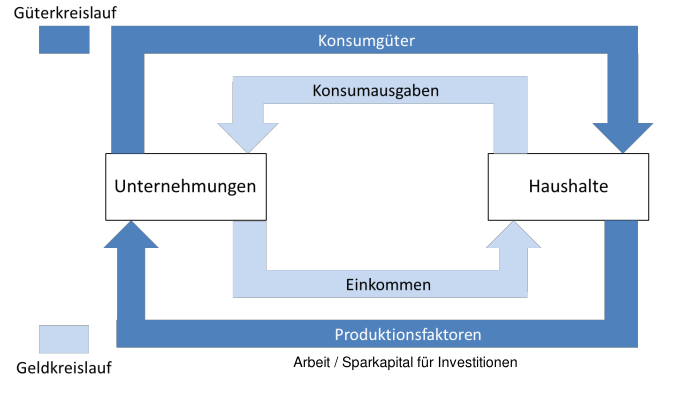
\includegraphics[width=.9\linewidth]{img/wirtschaftskreislauf.png}
\end{center}
\captionof{figure}{Der einfache Wirtschaftskreislauf}\label{fig:einfache-wirtschaftskreislauf}
}

\subparagraph{Der erweiterte Wirschaftskreislauf} \
\label{sec:org8e7f609}
{
\begin{center}
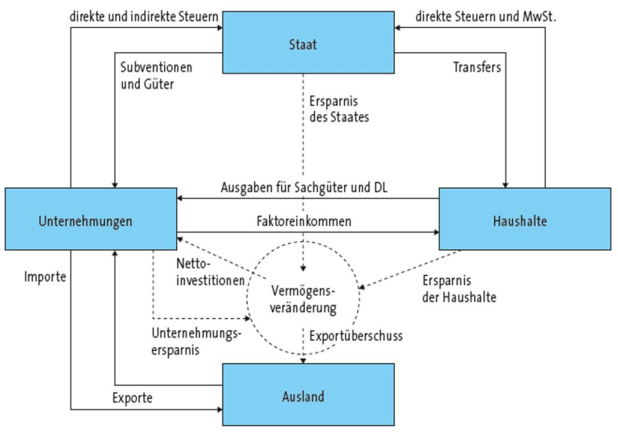
\includegraphics[width=.9\linewidth]{img/wirtschaftskreislauf_erweitert.png}
\end{center}
\captionof{figure}{Der erweiterte Wirschaftskreislauf}\label{fig:erweiterte-wirschaftskreislauf}
}

\subparagraph{Was ist Wohlstand} \
\label{sec:orgf24a098}
Wohlstand ist dasselbe wie das BIP (Bruttoinlandprodukt, \href{../../../roam/20220504151208-was_ist_das_bip.org}{Was ist das BIP?}).

\subparagraph{Was ist das BIP?} \
\label{sec:org22f4a12}
BIP ist nicht anders als Wohlstand (\href{../../../roam/20220504150706-was_ist_wohlstand.org}{Was ist Wohlstand?}).
Interessant: Beamtenlöhne entsprechen dem Produktionswert des Staats und fliesen daher ins BIP ein.


Das BIP gibt es als:
\begin{itemize}
\item Nominales BIP (Standard BIP = Produktionswert - Vorleistung)
\item Reales BIP (Referenzjahr)
\item BIP pro Kopf
\item Kaufkraftbereinigtes BIP (BIP auf einen internationalen Standard beglichen)
\end{itemize}

{
\begin{center}
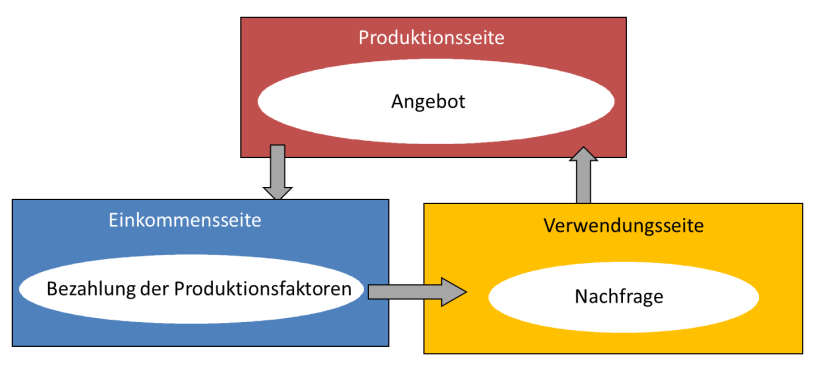
\includegraphics[width=.9\linewidth]{img/bip_blickwinkel.png}
\end{center}
\captionof{figure}{Die drei Blickwinkel des BIPs}\label{fig:drei-blickwinkel-bips}
}

\subparagraph{Die volkswirtschaftlichen Produktionsfaktoren} \
\label{sec:org7b35cfd}
\begin{itemize}
\item Arbeit - Menschen
\item Kapital - Maschine, Gebäuden, Infrastruktur
\item Technologien
\item Boden / natürliche Ressourcen
\end{itemize}

\section{Wachstum}
\label{sec:org0369339}
\subparagraph{Staatsquote} \
\label{sec:orgad4841a}
Die Staatsquote entspricht dem Verhältnis der Staatsausgaben zum BIP (\href{../../../roam/20220504151208-was_ist_das_bip.org}{Was ist das BIP?}).

\begin{equation}
\text{Staatsquote} = \frac{\text{Staatsausgaben}}{\text{BIP}}
\end{equation}

\subparagraph{Produktivität Schweiz} \
\label{sec:orge4f99c2}
\begin{itemize}
\item Wachstum der Staatsquote (\href{../../../roam/20220504151953-was_ist_die_staatsquote.org}{Was ist die Staatsquote?})
\item Abschottung des Binnenmarkts
\end{itemize}

Staatsquote: Weil die FaGe für weniger Betten zuständig ist, ist sie natürlich auch weniger produktiv.
Da FaGe meist vom Staat angestellt (Spitäler) ist der Staat nicht produktiv.

\section{Verteilung}
\label{sec:org26879fd}
\subparagraph{Pareto Effizienz} \
\label{sec:org545cfe0}
Eine Situation, ein Zustand oder ein Mark sind dann \emph{Pareto-effizient}, wenn es \textbf{nicht} möglich ist, die Situation eines einzelnen zu verbessern, ohne eine andere Person schlechter zu stellen.

\textbf{Beispiel}:
Eine Mutter wirft ihren zwei Kinder 8 Schokoriegeln zu.
Das eine Kinder fängt 2, das andere 6.
Die Situation ist \emph{Pareto-effizient}.
Wenn Kind 2 dem Kind 1 zwei Schokoriegeln gibt, hätten sie gleich viel.
Aber dem Kind 2 wurde etwas weggenommen.

\begin{quote}
Eine wirtschaftspolitische Massnahme ist dann effizient,
wenn sie die Situation eines Einzelnen verbessert, ohne andere schlechter zu
Stellen. Es gilt also, den Wohlstand in einem ersten Schritt insgesamt zu
vergrössern («ein grosser Kuchen lässt sich einfacher verteilen als ein kleiner
Kuchen»). - Daniel Aberer
\end{quote}

\subparagraph{Gini-Koeffizient} \
\label{sec:org00903d7}
Der Gini-Koeffizient ist ein Mass für die Ungleichverteilung von Einkommen oder Vermögen.
Je höher der Gini-Koeffizient ist, desto grösser ist die Ungleichverteilung.

\subparagraph{Gini-Koeffizient in der Schweiz} \
\label{sec:org70f1408}
In der Schweiz ist das Einkommen vor der Umverteilung ist schon relativ gleich.
Darum ist die Umverteilung (Gini-Koeffizient, \href{../../../roam/20220504154111-was_ist_der_gini_koeffizient.org}{Was ist der Gini-Koeffizient?}) relativ klein.


\begin{equation}
  \begin{aligned}
    CH_{min} &= 4000, CH_{max} = 16000 \\
    CH      &= \frac{CH_{max}}{CH_{min}} \\
	    &= \frac{16000}{4000} \\
	    &= 4
  \end{aligned}
\end{equation}

\begin{equation}
  \begin{aligned}
    DE_{min} &= 800, DE_{max} = 10000 \\
    DE &= \frac{DE_{max}}{DE_{min}} \\
    &= \frac{8000}{800} \\
    &= 10
  \end{aligned}
\end{equation}

\subparagraph{Vermögen vs. Einkommen} \
\label{sec:org3bf8cd1}
Das Einkommen das Geld, welches (monatlich) auf dem Lohnkonto landet.
Die direkte Bezahlung für meine Dienste.

Das Vermögen ist die Summe aller Wertgegenstände (Immobilien, finanzielle Vermögenswerte, Sachwerte, \ldots{})
Das Einkommen ist Teil des Vermögens.

\section{Makroökonomisches Modell}
\label{sec:orgd7e3e62}
\subparagraph{Das Makroökonomische Modell} \
\label{sec:org30cd618}
Das Makroökonomische Modell beschreibt, die Wirtschaftsleistung eines Landes.
Die Unternehmen erstellen die Güter, welche von den Haushalten, Unternehmen, Staat und Ausland nachgefragt werden.


\begin{description}
\item[{AA\textsubscript{L}}] Langfristigen aggregierten Angebotskurve = Kapazitätsgrenze
\item[{AA\textsubscript{K}}] Kurzfristige aggregierte Angebotskurve
\item[{AN}] Aggregierte Nachfragekurve
\end{description}

{
\begin{center}
\includegraphics[width=.9\linewidth]{img/makroökonomisches_gleichgewicht.png}
\end{center}
\captionof{figure}{Das Makroökonomische Model}\label{fig:das-makroökonomische-model}
}


Die \textbf{AN}-Kurve zeigt die Nachfrage nach Gütern.
Je tiefer das Preisniveau, desto höher die Nachfrage.

Die \textbf{AA\textsubscript{K}}-Kurve zeigt das Angebot an Gütern durch die Unternehmen auf.
Je höher das Preisniveau, desto höher das Güterangebot.
Kurzfristig bedeuted, dass die Produktionsfaktoren(\href{../../../roam/20220504150919-die_volkswirtschaftlichen_produktionsfaktoren.org}{Die volkswirtschaftlichen Produktionsfaktoren}) gleichbleiben.

Bei der Kapazitätsgrenze sind alle vorhandenend Produktionsfaktoren optimal ausgelasted (nicht maximal).
Man kann nich unbegrenz lange überhalt der Kapazitätsgrenze arbeiten.
Darum ist die Kurve nach der Grenze so steil.
Das entspräche einem Boom.

\subparagraph{Makroökonomisches Gleichgewicht} \
\label{sec:org460f785}
Das makroökonomische Gleichgewicht ist dann erreicht, wenn sich die Nachfrage (AN) und die Angebotskurve (AA\textsubscript{K}) am bei der Kapazitätsgrenze (AA\textsubscript{L}) schneiden.

Befindet man sich auf der Linken seite des Gleichgewichts entspricht das einer Rezession \(\rightarrow\) Arbeitslose, \ldots{}
Auf der rechten Seite ist der Boom, eine überhitze Wirtschaft.

{
\begin{center}
\includegraphics[width=.9\linewidth]{img/makroökonomisches_gleichgewicht.png}
\end{center}
\captionof{figure}{Makroökonomisches Gleichgewicht}\label{fig:makroökonomisches-gleichgewicht}
}

\section{Konjunktur}
\label{sec:org6c1f2ba}
\subparagraph{Phasen Konjunktur} \
\label{sec:org2d0b1dc}
\begin{description}
\item[{Rezession}] Abnahme des BIP während min. zwei aufeinanderfolgenden Quartalen
\end{description}

{
\begin{center}
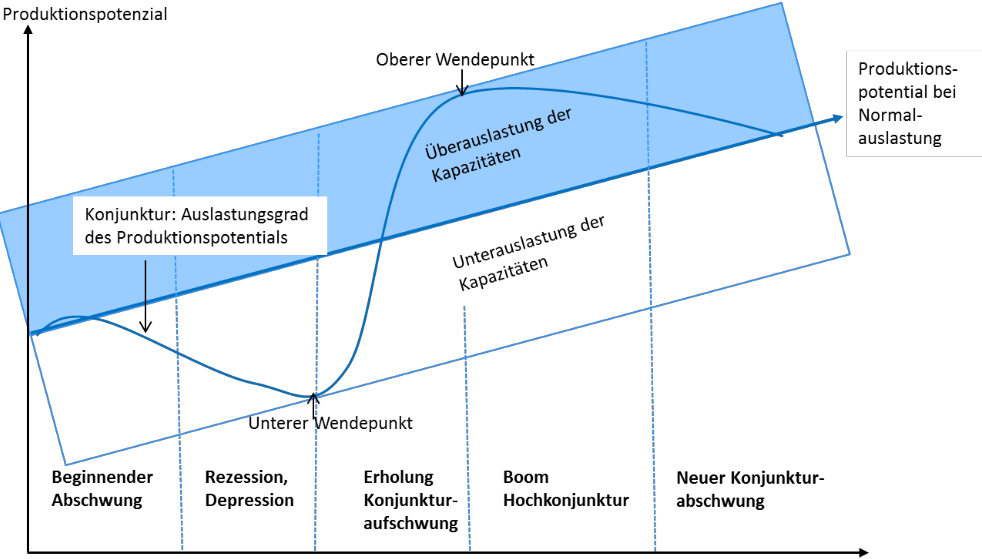
\includegraphics[width=.9\linewidth]{img/konjunktur_phasen.png}
\end{center}
\captionof{figure}{Die Phasen der Konjunktur}\label{fig:die-phasen-der-konjunktur}
}

\subparagraph{Veränderungen im makroökonomischen Modell} \
\label{sec:org7634d3e}
Alle Veränderungen im Modell (\href{../../../roam/20220614093525-was_ist_das_makrookonomische_modell.org}{Was ist das Makroökonomische Modell?}) haben einen Name, welcher wie folgt aufgebaut ist:
\begin{itemize}
\item (negativ|positiv) <Kurve>schock
\end{itemize}

Die Bedeutung:
\begin{description}
\item[{negativ}] links
\item[{positiv}] rechts
\item[{expansiv}] rechts
\item[{schock}] Bewegung findet statt
\end{description}


{
\begin{center}
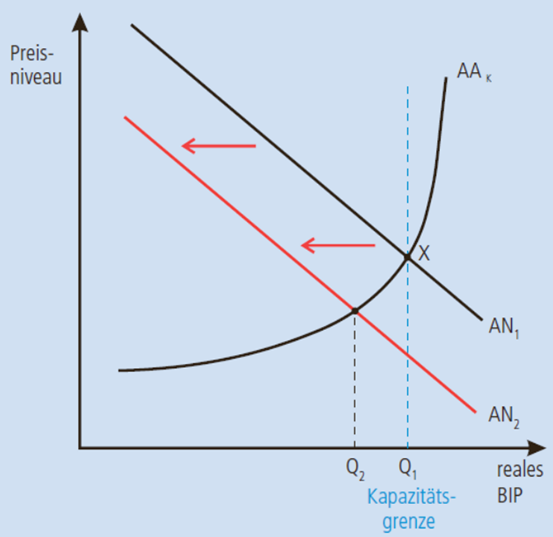
\includegraphics[width=.9\linewidth]{img/negative_nachfrageschock.png}
\end{center}
\captionof{figure}{Der negative Nachfrageschock}\label{fig:der-negative-nachfrageschock}
}


\begin{itemize}
\item Negative Nachfrageschock
\begin{itemize}
\item Niemand will etwas von der Schweiz kaufen
\end{itemize}
\item Positiver Nachfrageschock
\begin{itemize}
\item Alle wollen etwas von der Schweiz kaufen
\end{itemize}
\item Negativer Angebotsschock
\begin{itemize}
\item Kosten für Unternehmen gestiegen \(\leftarrow\) weniger produzieren
\end{itemize}
\item Positiver Angebotsschock
\begin{itemize}
\item Kosten für Unternehmen gesunken (meist durch verbesserte Technik) \(\leftarrow\) mehr produzieren
\end{itemize}
\end{itemize}

\subparagraph{Veränderung Gesamtangebot und -nachfrage} \
\label{sec:org19bde28}
\begin{itemize}
\item Rechtsverschiebung der Angebotsseite
\begin{itemize}
\item Tiefere Preise für natürliche Ressourcen
\item Tiefere Steuern für Unternehmen
\item Tiefere Lohnkosten
\item Effizientere Technologien
\end{itemize}
\end{itemize}


\begin{itemize}
\item Rechtsverschiebung der Nachfrageseite
\begin{itemize}
\item Höherer Konsum Haushalte (tiefere Sparzinsen / höheres Einkommen)
\item Höhere Investitionen der Unternehmen (tiefere Kreditzinsen)
\item Höhere Investitionen des Staats (Infrastrukturprojekte)
\item Höhere Konsum des Staats (Einstellung von Beamten)
\item Höhere Exporte
\item Tiefere Importe
\end{itemize}
\end{itemize}

\subparagraph{Konjunktur Zyklen} \
\label{sec:org61244d5}
Wenn der Ursprung das makroökonomische Gleichgewicht ist (\href{../../../roam/20220614100351-wann_ist_das_makrookonomische_gleichgewicht_erreicht.org}{Wann ist das makroökonomische Gleichgewicht erreicht?}) dann fallen wir mit einem:
\begin{itemize}
\item positivem Nachfrageschock in einen inflationären Boom
\item positivem Angebotsschock in einen deflationären Boom
\item negativem Nachfrageschock in eine Depression
\item negativem Angebotsschock in eine Stagflation
\end{itemize}


Heute bleibt man eigentlich nur noch auf der Inflationsseite (künstlich).
In der Depression gibt es auch die Deflationsfalle, aus der man nicht mehr / schwer herauskommt.
Diese möchte man vermeiden.


{
\begin{center}
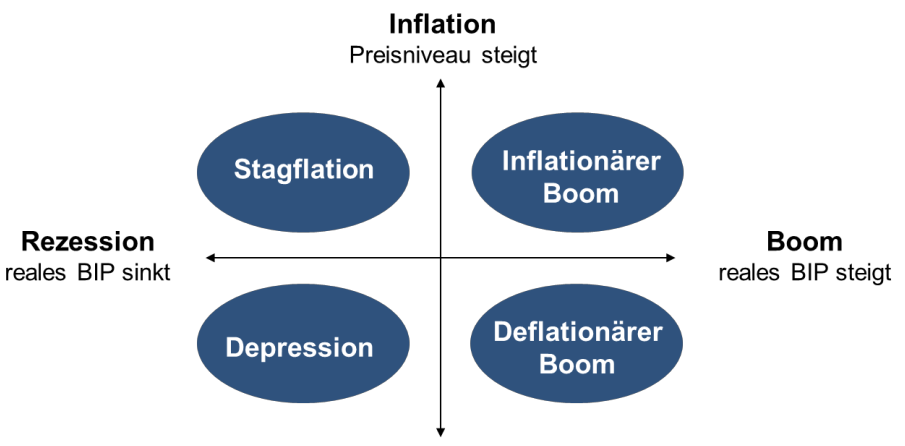
\includegraphics[width=.9\linewidth]{img/konjunkturzyklen.png}
\end{center}
\captionof{figure}{Konjunkturzyklen}\label{fig:konjunkturzyklen}
}

\subparagraph{Verschiedene Arten Arbeitslosigkeit} \
\label{sec:org4b14ee5}
Es gibt in der Schweiz zwei Arten von Arbeitslosigkeit:
\begin{itemize}
\item Konjunkturelle Arbeitslosigkeit (Y in \ref{fig:die-beveridge-kurve})
\item Sockelarbeitslosigkeit (X in \ref{fig:die-beveridge-kurve})
\end{itemize}


{
\begin{center}
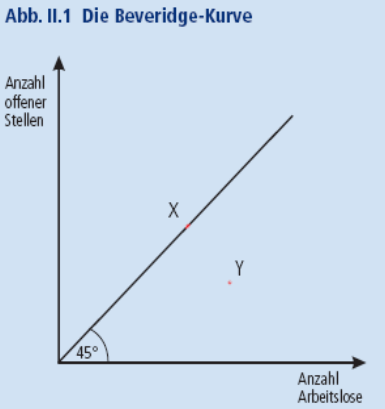
\includegraphics[width=.9\linewidth]{img/beveridge_kurve.png}
\end{center}
\captionof{figure}{Die Beveridge-Kurve}\label{fig:die-beveridge-kurve}
}

\subparagraph{Konjunkturelle Arbeitslosigkeit} \
\label{sec:org5c30741}
Konjunkturelle Arbeitslosigkeit ist dann, wenn es mehr Personen gibt, welche Arbeit suchen, als es offene Stellen gibt (Y in \ref{fig:die-beveridge-kurve}).

{
\begin{center}
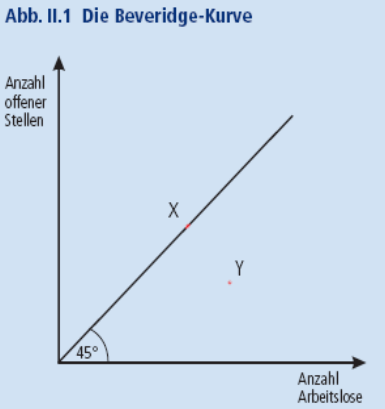
\includegraphics[width=.9\linewidth]{img/beveridge_kurve.png}
\end{center}
\captionof{figure}{Die Beveridge-Kurve}\label{fig:die-beveridge-kurve}
}

\subparagraph{Konjunkturpolitiken} \
\label{sec:org095d2d5}
Es gibt drei Möglichkeiten, um die Konjunktur zu lenken:
\begin{enumerate}
\item "Nichts tun":
\begin{itemize}
\item Der Markt regelt es das schon
\end{itemize}
\item Aktive \textbf{keynesianische} Konjunkturpolitik
\begin{itemize}
\item Staat fördert aktive die gesamtwirtschaftliche Nachfrage durch Fiskal-/ und Geldpolitik (Positiver Nachfrageschock)
\end{itemize}
\item Stärkung der automatischen Stabilisatoren
\begin{itemize}
\item Staatliche Einnahmen und Ausgaben, die die Nachfrage automatisch stimuliert, wenn die gesamtwirtschaftliche Nachfrage zurück geht
\end{itemize}
\end{enumerate}

\section{Preisstabilität}
\label{sec:orgae0597d}
\subparagraph{Inflation} \
\label{sec:org0324c73}
Inflation ist eine permanente Steigerung des Preisniveaus.
Auslöser einer Inflation ist eine einmalige Steigerung des Preisniveaus.
Wenn die Haushalte und Unternehmen davon ausgehen, das das Preisniveau weiter steigt, wird man in eine Inflation fallen.
Heute konnte ich mit 1 CHF zwei Brot kaufen, wenn ich warte, kann ich morgen nur noch ein Brote für 1 CHF kaufen.


\subparagraph{Lohn-Preis-Spirale} \
\label{sec:org7724142}
Die Lohn-Preis-Spirale führt zu einer Inflation.

\begin{enumerate}
\item Sinkende Reallöhne der Haushalte (z.B. weil Preise gestiegen sind)
\item Diese fordern (wegen Inflationserwartungen) eine Steigerung der Nominallöhne, welche die Erhöhung des Preisniveaus überkompensieren
\item Damit ergibt sich eine Steigerung der Reallöhne
\item Dies bedeutet für die Unternehmen eine Kostensteigerung
\item Die Unternehmen werden deshalb höhere Güterpreise verlangen
\item Damit erhöht sich wieder das Preisniveau -> Go to 1
\end{enumerate}

\subparagraph{Geldpolitik Zentralbank und Inflation} \
\label{sec:org47d4371}
Die link Seite entspricht der Güterwirtschaft (nominales BIP).
Die rechte Seite entspricht der Geldwirtschaft.

\begin{equation}
  \label{eqn:quantitaetsgleichung}
  \begin{align}
    \text{Preisniveau} \cdot \text{reales BIP} &= \text{Geldmenge} \cdot \text{Geldumlaufgeschwindigkeit} \\
    \text{nominales BIP} &= \text{Geldmenge} \cdot \text{Geldumlaufgeschwindigkeit} \\
    P \cdot Q &= M \cdot V
  \end{align}
\end{equation}

V = Umlaufgeschwindigkeit des Geldes (Anzahl Verwendungen einer Geldeinheit pro Jahr).
V kann nicht gemessen werden!
V kann nur berechnet werden, wenn die anderen drei Grössen bekannt sind.



\subparagraph{Expansive Geldpolitik} \
\label{sec:org1cd50dc}
\begin{itemize}
\item Fall 1:
\begin{itemize}
\item \(\Delta P < \Delta Q\)
\end{itemize}
\item Fall 2:
\begin{itemize}
\item \(\Delta P > \Delta Q\)
\end{itemize}
\end{itemize}

{
\begin{center}
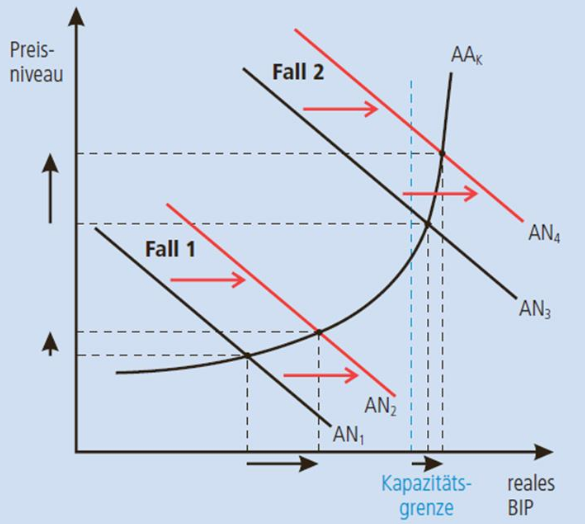
\includegraphics[width=.9\linewidth]{img/inflationswirkung_expansiver_geldpolitik.png}
\end{center}
\captionof{figure}{Inflationswirkung expansiver Geldpolitik}\label{fig:inflationswirkung-expansiver-geldpolitik}
}

\subparagraph{Deflation} \
\label{sec:org97aeda3}
Deflation bedeutet ein permanenter Rückgang des Preisniveaus.
Deflation ist dann schädlich, wenn diese auf einem Rückgang der aggregierten Nachfrage (AN) beruht (\href{../../../roam/20220614093525-was_ist_das_makrookonomische_modell.org}{Was ist das Makroökonomische Modell?}).

\section{Markt und Preise}
\label{sec:orge965929}
\subparagraph{Verschiedene Volkswirtschaften} \
\label{sec:orgd2c86e7}
Es gibt zwei Arten, wie eine Volkswirtschaft organisiert werden kann:
\begin{itemize}
\item Planwirtschaft
\begin{itemize}
\item Alle Ressourcen gehören dem Staat
\item Zentrale Planungsbehörde lenkt den Einsatz der Ressourcen
\end{itemize}
\item Marktwirtschaft
\begin{itemize}
\item Ressourcen gehören privaten Haushalten / Firmen
\item Private Haushalte / Firmen entscheiden über Ressourceneinsatz
\end{itemize}
\end{itemize}

\subparagraph{Mikroökonomisches Modell} \
\label{sec:orgaaaf4a0}

\begin{itemize}
\item K-Rente: Konsumentenrente = Zahlungsbereitschaft des Käufers, abzüglich des Preises, den er tatsächlich bezahlt
\begin{itemize}
\item Konsumenten würden auch mehr zahlen, zahlen aber nur den Marktpreis
\end{itemize}
\item P-Rente: Produzentenrente = Erlös des Verkäufers, abzüglich der Kosten, die für Erwerb / Herstellung entstanden sind
\begin{itemize}
\item Produzenten würden auch günstiger verkaufen, aber verkaufen zum Marktpreis
\end{itemize}
\item Wohlfahrt: Gesamte Rente = K-Rente = P-Rente
\end{itemize}

{
\begin{center}
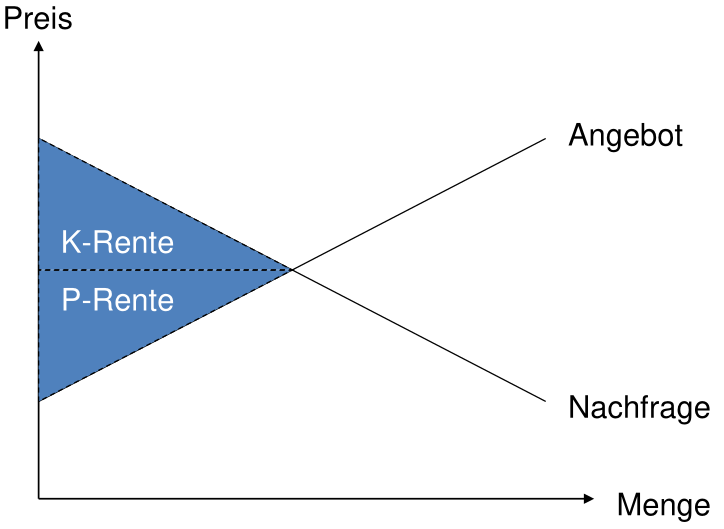
\includegraphics[width=.9\linewidth]{img/mikrooekonomische_grundmodell.png}
\end{center}
\captionof{figure}{Mikroökonomische Grundmodell}\label{fig:mikroökonomische-grundmodell}
}


\subparagraph{Mindestpreis} \
\label{sec:org6983f93}
Durch das Setzen eines Mindestpreises, entsteht Wohlfahrtsverlust.
Zusätzlich gibt es mehr Angebot als Nachfrage.

{
\begin{center}
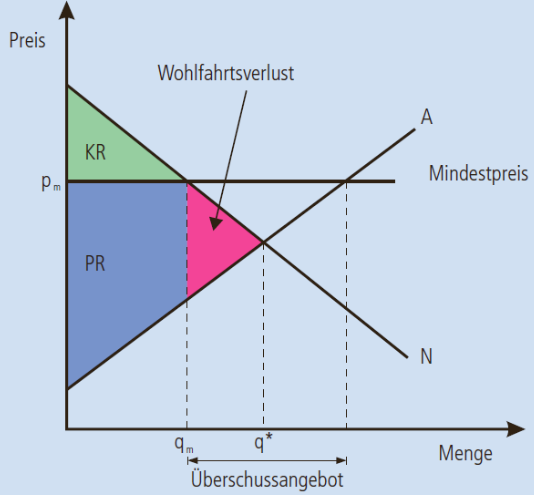
\includegraphics[width=.9\linewidth]{img/mindestpreis.png}
\end{center}
\captionof{figure}{Mindestpreis}\label{fig:mindestpreis}
}

\subparagraph{Höchstpreis} \
\label{sec:org1b72a8e}

Durch das Setzten eines Höchstpreises entsteht Wohlfahrtsverlust.
Zusätzlich gibt es mehr Nachfrage als Angebot.

{
\begin{center}
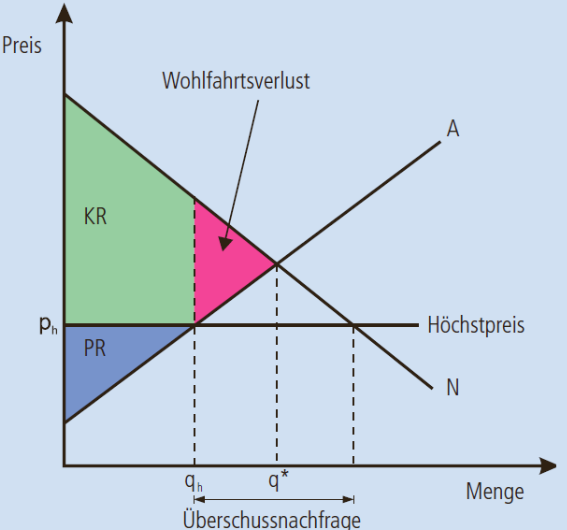
\includegraphics[width=.9\linewidth]{img/hoechstpreis.png}
\end{center}
\captionof{figure}{Höchstpreise}\label{fig:hoechstpreise}
}

\subparagraph{Preiselastizität} \
\label{sec:orgdb632e0}
Je kleiner desto unelastischer.
\begin{equation}
  \label{eqn:preielastizitaet}
  \text{Preiselastizität der Nachfrage} = \frac{\text{Veränderung der nachgefragten Menge in \%}}{\text{Veränderung des Preises in \%}}
\end{equation}

Es gibt \textbf{unelastische Nachfrage} und \textbf{elastische Nachfrage}.
Lebenswichtige Güter (Wasser, Brot, \ldots{}) sind unelastisch.
Das heisst, es benötigt eine (sehr) grosse Änderung des Preises, um eine Reaktion auszulösen.

Hingegen Güter wie Lippenstifte sind elastisch.
Wenn der Preis leicht steigt, gibt eine (sehr) starke Nachfrageeinbussen.

\section{Arbeitsmarkt}
\label{sec:org601b772}
\subparagraph{Arbeitsmarkt mikroökonomisch} \
\label{sec:orgae21108}
\begin{enumerate}
\item Unternehmen bieten \(\ge\) Marktlohn an. Ihre Nachfrage nach Arbeitskräften wird erfüllt
\item Arbeitskräfte erhalten kein Arbeitsangebot, da sie nicht bereits sind zum Marktlohn zu arbeiten
\item Arbeitskräfte erhalten Arbeitsangebot, da sie bereits sind \(\le\) Marktlohn zu arbeiten
\item Unternehmen bieten < Marktlohn an. Ich Nachfrage nach Arbeitskräfte wird nicht erfüllt
\end{enumerate}


Wichtig: Die Arbeitnehmer im Abschnitt 2 sind \textbf{NICHT} arbeitslos.
Diese könnten arbeiten, wenn sie den Marktpreis akzeptieren würden.

{
\begin{center}
\includegraphics[width=.9\linewidth]{img/arbeitsmarkt_mikroökonomisch.png}
\end{center}
\captionof{figure}{Arbeitsmarkt als mikroökonomisches Modell}\label{fig:arbeitsmarkt-als-mikroökonomisches-modell}
}

\subparagraph{Messung Arbeitslosigkeit} \
\label{sec:org8c33624}
Als Arbeitslos gilt, wer zwischen 15 und 64 Jahren ist, arbeiten möchte, aber keine Arbeit findet.
Studenten sind daher nicht Arbeitslos, sondern gehören zu der Nichterwerbsbevölkerung.

Die Anzahl Arbeitslosen werden darüber gemessen, wer sich bis Ende Monat beim RAV meldet.
Wenn man ausgesteuert ist, bekommt man kein Geld mehr, aber gilt immer noch als Arbeitslos.
Es gibt aber den Fall, dass diese nicht mehr zum RAV kommen.
Diese werden dann versucht über Telefonumfrage, etc. zu ermittelt.

\begin{equation}
  \label{eqn:arbeitslosenquote}
  \text{Arbeitslosenquote} = \frac{\text{Arbeitslose}}{\text{Erwerbsbevölkerung}} \times 100 \\
\end{equation}

\begin{equation}
  \label{eqn:erwerbsquote}
  \text{Erwerbsquote} = \frac{\text{Erwerbsbevölkerung}}{\text{15- bis 64-Jährige}} \times 100 \\
\end{equation}

\begin{equation}
  \label{eqn:erwerbstaetigenquote}
  \text{Erwerbstätigenquote} = \frac{\text{Beschäftigte}}{\text{15- bis 64-Jährige}} \times 100 
\end{equation}


{
\begin{center}
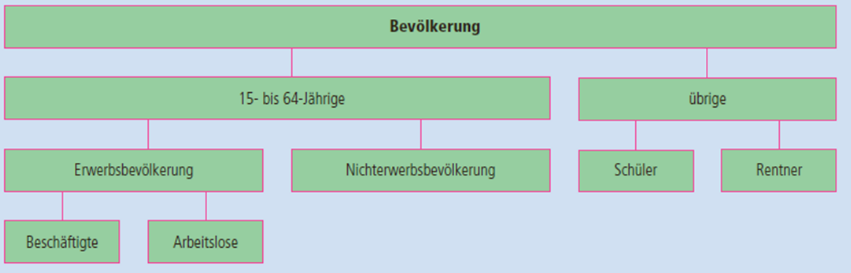
\includegraphics[width=.9\linewidth]{img/arbeitslosigkeit_aufbau_bevoelkerung.png}
\end{center}
\captionof{figure}{Zusammensetzung der Bevölkerung}\label{fig:zusammensetzung-der-bevölkerung}
}

\subparagraph{Sockelarbeitslosigkeit} \
\label{sec:org526bac1}
\begin{quote}
Anzahl der offenen Stellen ist gleich gross
oder grösser als die Anzahl der Arbeitslosen.
 -- Daniel Aberer
\end{quote}

Die Sockelarbeitslosigkeit ist in den letzten Jahren gestiegen.

Ab den 1990er Jahren begannen Frauen auch nach der Heirat weiterzuarbeiten.
Das führte zu einem starken Anstieg des Arbeitskräfteangebots.
Aber die Nachfrage ist gleichgeblieben.

Ursprünglich konnten die Ausländer für 9 Monat arbeiten, 3 Monate mussten sie nach Hause.
Dies wurde angepasst und sie konnten bleiben.
Währen dem Winter (3 Monate) erhalten sie nun Arbeitslosengeld, weil die Baustellen ja trotzdem geschlossen sind.

\section{Geld}
\label{sec:org3d7d941}
\subparagraph{Was ist Geld?} \
\label{sec:org245d275}
Ich produziere nicht alle Güter, die ich benötige (Arbeitsteilung).
Ich tausche Geld gegen ein fremdes Gut.
Das Geld soll den Tauschhandel vereinfachen.

Geld hat drei Funktionen:
\begin{enumerate}
\item Zahlungsmittel (siehe oben)
\item Masseinheit (Vergleichbarkeit von Gütern)
\item Wertaufbewahrungsmittel
\end{enumerate}

\subparagraph{Verschiedene Geldmenge} \
\label{sec:org45057ad}
In der Wirtschaft spricht man von M0, M1, M2 und M3.
Die Zentralbank (z.B. die SNB) erschafft das M0 durch die Offenmarktpolitik (\href{../../../roam/20220615113801-was_ist_die_offenmarktpolitik.org}{Was ist die Offenmarktpolitik?}).
M1, M2 und M3 wird von den Geschäftsbanken erschaffen durch Kreditvergaben.

\begin{figure}[H]
  \centering
  \begin{subfigure}{0.4\textwidth}
    \centering
    \includegraphics[width=3in]{img/geldschöpfung_overview.png}
    \caption{Geldschöpfung Überblick \label{fig:geldschöpfung-ueberblick}}
  \end{subfigure}
  \hfill
  \begin{subfigure}{0.4\textwidth}
    \centering
    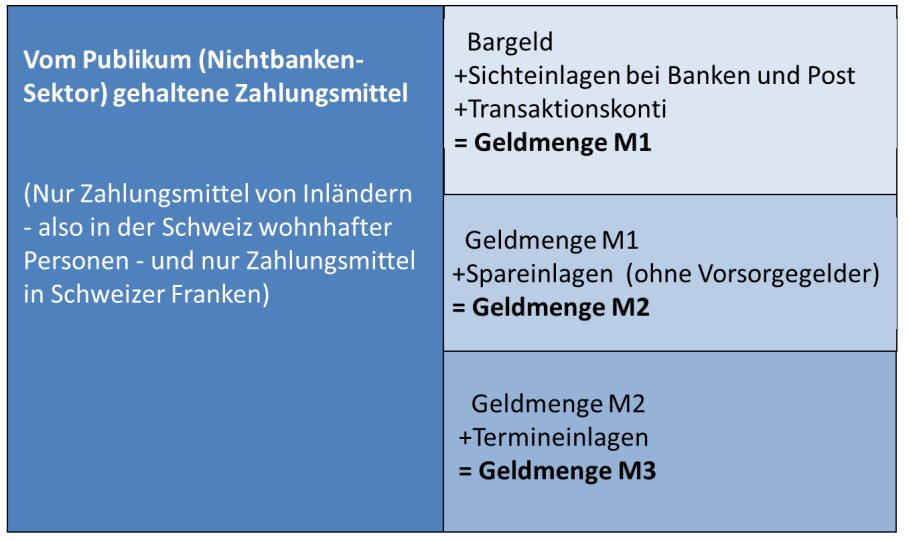
\includegraphics[width=3in]{img/geldmenge_m1_m2_m3.png}
    \caption{Geldmenge M1, M2, M3 \label{fig:geldmenge-m1-m2-m3}}
  \end{subfigure}
  \caption{
    \label{fig:gelschöpfung}
    Geldschöpfung
  }
\end{figure}

\subparagraph{Bilanz der SNB} \
\label{sec:orgd8efa84}
{
\begin{center}
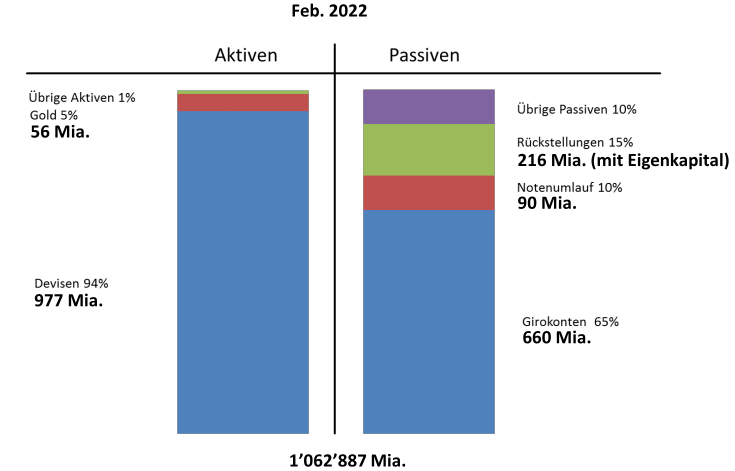
\includegraphics[width=.9\linewidth]{img/bilanz_snb.png}
\end{center}
\captionof{figure}{Bilanz der SNB}\label{fig:bilanz-der-snb}
}

\subparagraph{Offenmarktpolitik} \
\label{sec:org5a68579}

Die Zentralbank (z.B. SNB) kauft und verkauft Aktiva (vor allem Wertschriften) an inländische Geschäftsbanken.
Damit erschafft / vernichtet die Zentralbank M0.

Die Nationalbank zahlt die Aktiva mit "frisch gedruckten" Geld, welches den Girokonten der Geschäftsbanken gutgeschrieben wird.

\subparagraph{Aufträge Zentralbank} \
\label{sec:orgaf66624}
Die Zentralbank hat keine Gewinnziele.
Stattdessen kann die Zentralbank andere Ziele haben:

\begin{enumerate}
\item Wechselkursziele:
\begin{itemize}
\item Fixierung des Wechselkurses an internationale Währung
\end{itemize}
\item Geldmengenziele:
\begin{itemize}
\item Monetaristischer Ansatz: \(P \time Q = M \time V\) (\href{../../../roam/20220614170056-wie_sieht_der_theoretische_zusammenhang_zwischen_der_geldpolitik_der_zentralbank_und_der_inflation_aus.org}{Wie sieht der theoretische Zusammenhang zwischen der Geldpolitik der Zentralbank und der Inflation aus?})
\end{itemize}
\item Inflationsziele:
\begin{itemize}
\item Wahrung der Preisstabilität
\end{itemize}
\end{enumerate}

\section{Wechselkurs}
\label{sec:org2fc6496}
\subparagraph{Wechselkurs mikroökonomisch} \
\label{sec:org41706e5}
Der Wechselkurs kann auch im mikroökonomischen Modell dargestellt werden.
Beispiele für Nachfragen nach Schweizer Franken währen:
\begin{itemize}
\item Exporte
\item Arbeits- und Kapitalerträge
\end{itemize}

Beispiele für Angebote von Schweizer Franken währen:
\begin{itemize}
\item Importe
\item Devisenkäufe der SNB
\end{itemize}


{
\begin{center}
\includegraphics[width=.9\linewidth]{img/wechselkurse_mikroökonomisch.png}
\end{center}
\captionof{figure}{Wechselkurse als mikroökonomisches Modell}\label{fig:wechselkurse-als-mikroökonomisches-modell}
}

\subparagraph{Wechselkursarten} \
\label{sec:org309f119}
Es gibt zwei Wechselkurse:
\begin{itemize}
\item nominaler Wechselkurs (\href{../../../roam/20220615143018-was_ist_der_nominale_wechselkurs.org}{Was ist der nominale Wechselkurs?})
\item realer Wechselkurs (\href{../../../roam/20220615150048-was_ist_der_reale_wechselkurs.org}{Was ist der reale Wechselkurs?})
\end{itemize}

\subparagraph{Nominaler Wechselkurs} \
\label{sec:org0a14fb3}
Der nominale Wechselkurs ist das Verhältnis der inländischen Währung im Vergleich zur ausländischen Währung.
Wenn der norminale Wechselkurs e steigt, entspricht das einer Abwertung der inländischen Währung.

\begin{equation}
  \label{eqn:nominaler-wechselkurs}
  \text{e (nominaler Wechselkurs)} = \frac{\text{inländische Währung}}{\text{ausländische Währung}} = \frac{\text{CHF}}{\text{EUR}}
\end{equation}

\subparagraph{Realer Wechselkurs} \
\label{sec:org0ecf719}
Der reale Wechselkurs beschreibt, wie viele Güter ich mit meinem Geld im Ausland kaufen kann.
Das heisst, die unterschiedlichen Preisniveaus werden berücksichtigt.

\(p\) entspricht dem Preisniveau (siehe \href{../../../roam/20220614170056-wie_sieht_der_theoretische_zusammenhang_zwischen_der_geldpolitik_der_zentralbank_und_der_inflation_aus.org}{Quantitätsgleichung}).

\begin{equation}
  \label{eqn:realer-wechselkurs}
  \begin{align}
  \text{r (realer Wechselkurs)} &= \frac{e \times p \times \text{Preis Güterkorb im Ausland in ausländischer Währung}}{p \times \text{Preis Güterkorb im Inald in inländischer Währung}} \\
    r &= \frac{e \times \text{Inflation Ausland}}{\text{Inflation Inland}}
  \end{align}

\end{equation}

\subparagraph{Effekte Geldpolitik auf Wechselkurs} \
\label{sec:orga18c0d3}
Wenn die inländische Geldmenge vergrössert wird, steigt der nominale Wechselkurs (\href{../../../roam/20220615143018-was_ist_der_nominale_wechselkurs.org}{Was ist der nominale Wechselkurs?}) sofort.
Das Preisniveau im Inland aber nicht.
Der reale Wechselkurs (\href{../../../roam/20220615150048-was_ist_der_reale_wechselkurs.org}{Was ist der reale Wechselkurs?}) steigt ebenfalls.

Langfristig passt sich das Preisniveau im Inland an.
Der reale Wechselkurs bleibt langfristig gesehen gleich.


{
\begin{center}
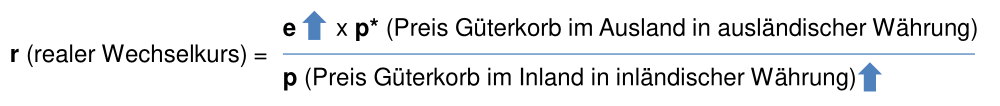
\includegraphics[width=.9\linewidth]{img/langfritiger_effekt_realer_wechselkurs.png}
\end{center}
\captionof{figure}{Langfristige Effekte}\label{fig:langfristige-effekte}
}

\section{Staatsfinanzen}
\label{sec:orgd0afa96}
\subparagraph{Staatseinkommen} \
\label{sec:org309426a}
Der Staat hat drei Möglichkeiten Einnahmen zu generieren:
\begin{enumerate}
\item Steuern
\begin{itemize}
\item Direkte Steuern (entsprechen 2/3 der Staatseinnahmen)
\item Indirekte Steuern (MWST)
\item Gebühren
\end{itemize}
\item Verschuldung
\begin{itemize}
\item Deckung von Investitionen
\item Staatskonsum
\end{itemize}
\item Inflationssteuer
\begin{enumerate}
\item Ausweitung der Geldmenge
\end{enumerate}
\end{enumerate}


{
\begin{center}
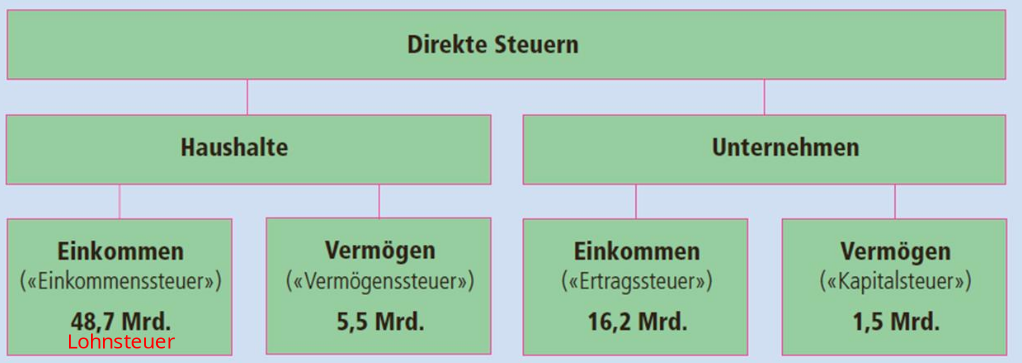
\includegraphics[width=.9\linewidth]{img/staatseinnahmen_schweiz.png}
\end{center}
\captionof{figure}{Aufteilung der Steuern}\label{fig:aufteilung-der-steuern}
}

\subparagraph{Vor- und Nachteile Staatsverschuldung} \
\label{sec:org67bb51f}
Nachteile:
\begin{itemize}
\item Wenn sich der Staat im Inland verschuldet, führt das zum Rückgang der inländischen Investitionen der Unternehmen.
\item Wenn sich der Staat im Ausland verschuldet, führt das zum Rückgang der Exporte.
\end{itemize}

Vorteile:
\begin{itemize}
\item langfristige Projekte können durch die zukünftige Generation finanziert werden
\item Der Staat kann konjunkturelle Schwankungen (\href{../../../roam/20220614102344-die_phasen_der_konjunktur.org}{Die Phasen der Konjunktur}) durch Veränderung der Nachfrage ausgleichen (keynesianische Politik, \href{../../../roam/20220614161544-die_verschiedenen_konjunkturpolitiken.org}{Die verschiedenen Konjunkturpolitiken})
\end{itemize}

\subparagraph{Fiskalquote} \
\label{sec:org561d2cc}
Die Fiskalquote beschreibt den Anteil der Steuereinnahmen am realen BIP (\href{../../../roam/20220504151208-was_ist_das_bip.org}{Was ist das BIP?}).

\subparagraph{Schuldenbremse} \
\label{sec:org520a069}
\begin{enumerate}
\item Jedes Jahr wird ein Einnahmebudget definiert (konservativ, eher zu wenig berechnet)
\item Das Ausgabenbudget entspricht dem Einnahmebudget
\item Meistens kommt es aber besser als erwartet (die Einnahmen sind höher als budgetiert).
\item Nachträglich darf das Ausgabenbudget nicht erhöht werden, d.h. es entstehen Überschüsse
\end{enumerate}


Durch das Einführen der Schuldenbremse, baut der Schweizer Staat stetig die Schulden ab.

\section{{\bfseries\sffamily TODO} Internationale Arbeitsteilung}
\label{sec:org16e4f08}
\subparagraph{Prinzip des kompartiven Kostenvorteils} \
\label{sec:org413b69e}

\begin{quote}
Internationale Arbeitsteilung bringt positive Wohlfahrtseffekte, unabhängig
davon, ob der Weltmarktpreis eines Gutes höher oder tiefer als der
entsprechende Heimmarktpreis ist.
\end{quote}

{
\begin{center}
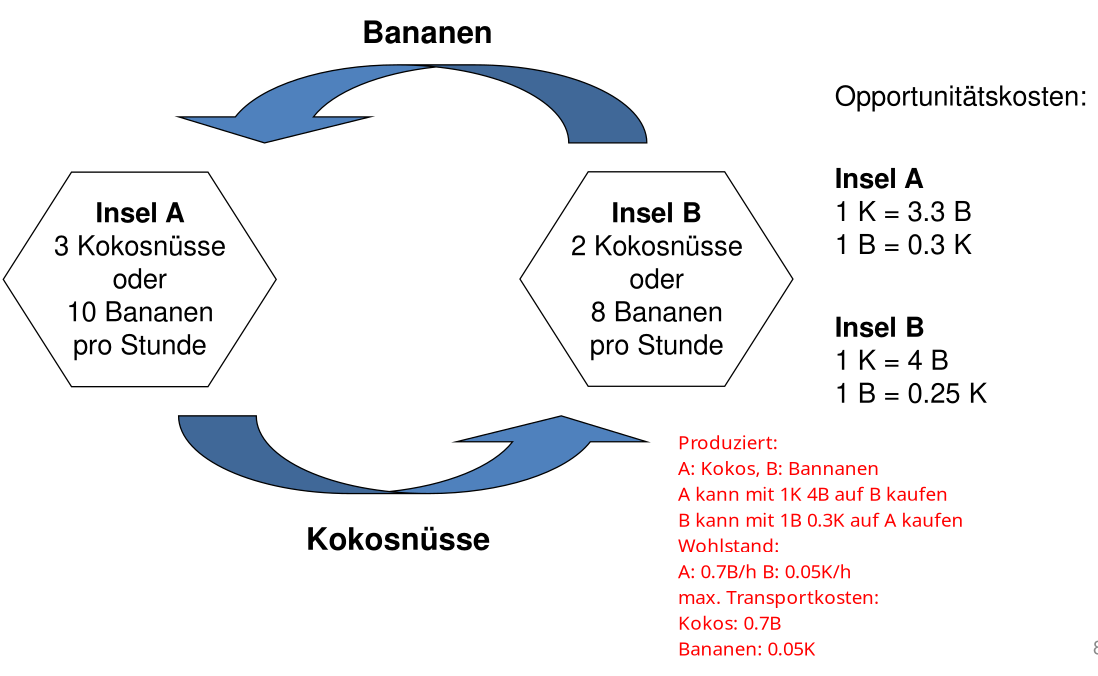
\includegraphics[width=.9\linewidth]{img/komparativen_kostenvorteils.png}
\end{center}
\captionof{figure}{Komparativen Kostenvorteil}\label{fig:komparativen-kostenvorteil}
}

\subparagraph{Wohlfahrt} \
\label{sec:org6bc1954}
Die Wohlfahrt entspricht der Summe aus der Konsumentenrente und der Produzentenrente.
In Figure \ref{fig:wohlfahrt-bei-autarkie} entspricht das dem blauen Dreieck.

{
\begin{center}
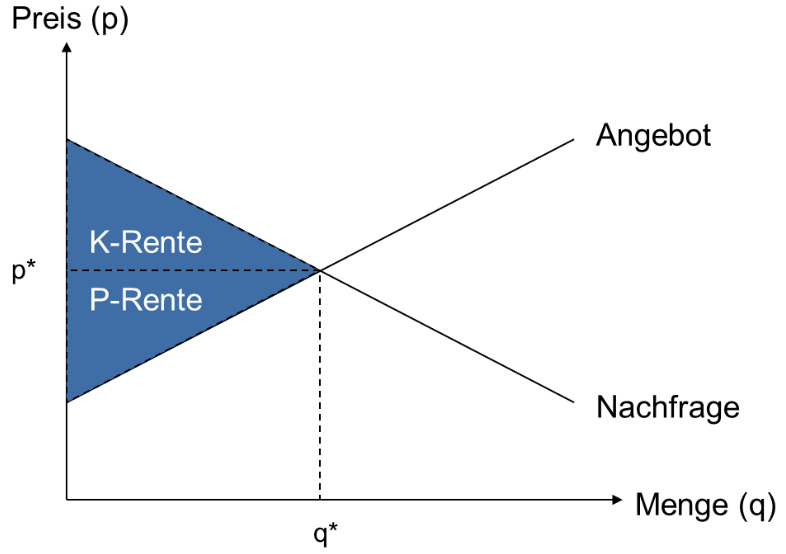
\includegraphics[width=.9\linewidth]{img/wohlfahrt_bei_autarkie.png}
\end{center}
\captionof{figure}{Wohlfahrt bei Autarkie}\label{fig:wohlfahrt-bei-autarkie}
}

\subparagraph{Wohlfahrtseffekte} \
\label{sec:orgf47922a}

Wie die Figure \ref{fig:mit-zoelle} zeigt, sind Zölle keine gute Idee.
Sie vermindern die Wohlfahrt.
\begin{figure}[H]
  \centering
  \begin{subfigure}{0.4\textwidth}
    \centering
    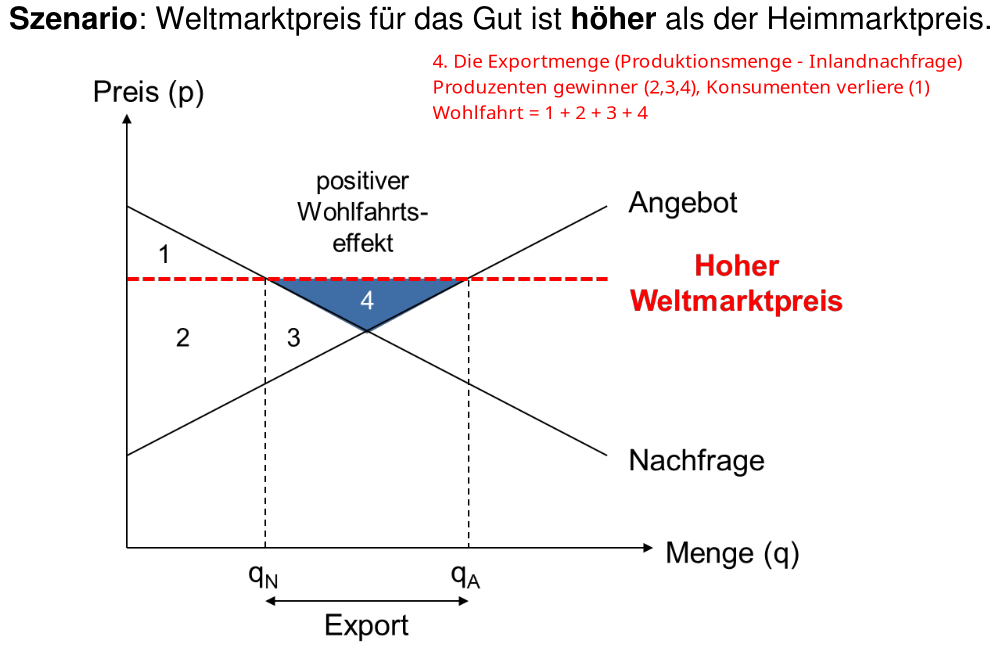
\includegraphics[width=3in]{img/wohlfahrt_hoher_welkmakrspreis.png}
    \captionof{figure}{Hoher Weltmarktpreis \label{fig:hoher-preis}}
  \end{subfigure}
  \hfill
  \begin{subfigure}{0.4\textwidth}
    \centering
    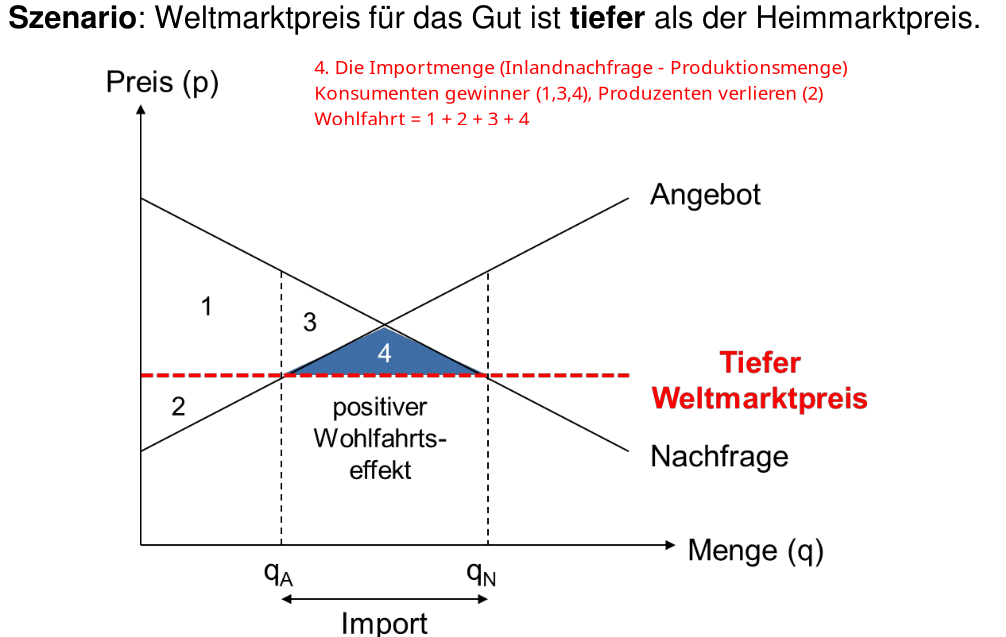
\includegraphics[width=3in]{img/wohlfahrt_tiefer_weltmarktpreis.png}
    \captionof{figure}{Tiefer Weltmarktpreis \label{fig:tiefer-preis}}
  \end{subfigure}
  \vfill
  \begin{subfigure}{0.4\textwidth}
    \centering
    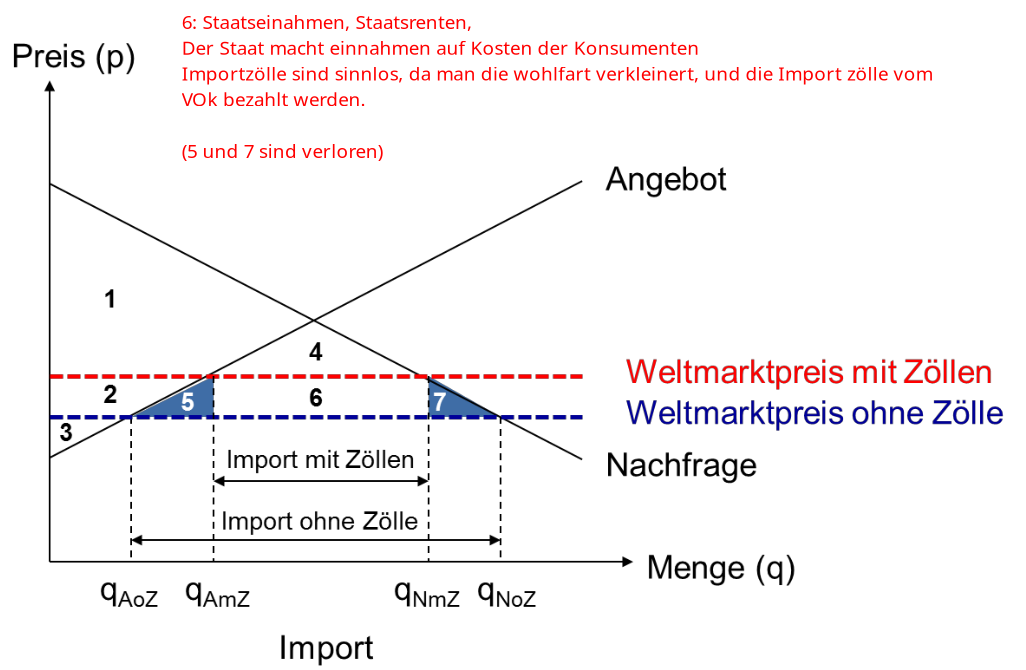
\includegraphics[width=3in]{img/wohlfahrt_zoelle.png}
    \captionof{figure}{
      Zölle
      \label{fig:mit-zoelle}
    }
  \end{subfigure}
  \caption{
    \label{fig:wohlfahrt-effekte}
    Wohlfahrteffekte
  }
\end{figure}

\subparagraph{Formen des Protektionsimus} \
\label{sec:orgfd852df}

Importzölle haben negative Auswirkungen auf die Wohlfahrt (\href{../../../roam/20220622110833-die_verschiedenen_wohlfahrseffekte.org}{Die verschiedenen Wohlfahrseffekte}) und sind daher \textbf{nicht} zu empfehlen.
Es gibt aber alternativen, um den inländischen zu schützen:

\begin{itemize}
\item Quoten
\item Technische Handelshemmnisse
\item Subventionen
\item Öffentliche Aufträge (Bevorzugung von Inländer)
\end{itemize}

\subparagraph{Handelsliberalisierungen} \
\label{sec:orgc7d4763}

Es werden drei Formen von internationaler Arbeitsteilung unterschieden:
\begin{itemize}
\item Multilaterale Handelsliberalisierung (z.B. WTO)
\item Regionale Handelsliberalisierung (z.B. EU)
\item Bilaterale Handelsliberalisierung (der "Schweizer" Weg)
\end{itemize}

\subparagraph{Effekte der Regionalen Integration} \
\label{sec:orgd08304f}
Durch regionale Handelsliberalisierungen (z.B. EU) entsteht eine Diskriminierung der Länder, welche nicht in diesem Integrationsraum ist (z.B. die Schweiz).
Dadurch entstehen zwei Effekte:
\begin{itemize}
\item Handelsschaffung
\item Handelsumlenkung
\end{itemize}


Handelsschaffung heisst, dass zwischen zwei Parteien (A und B) mehr Handel generiert wird.
Zusätzlich wird der Handel mit Land C umgelenkt zu B.
Das passiert, weil A und B keine Zölle mehr haben.
Daher ist für A, B immer günstiger, da C immer noch Zölle hat.


{
\begin{center}
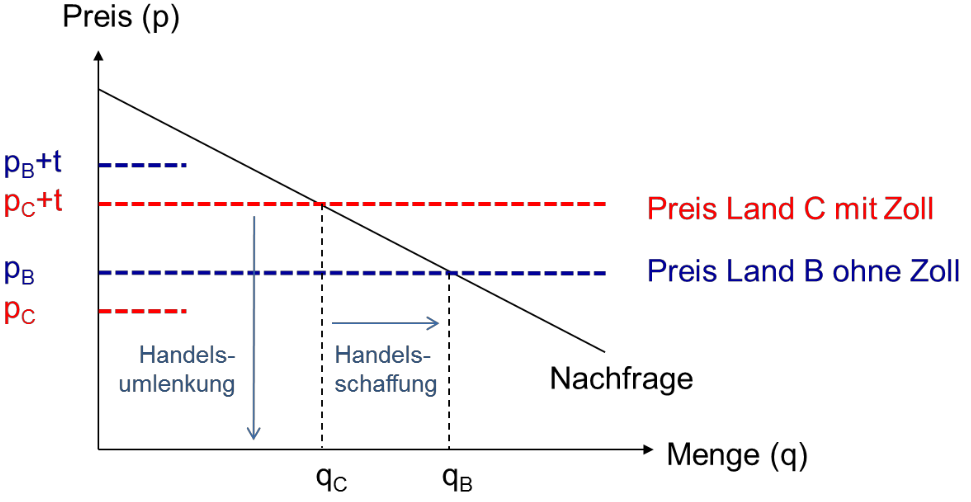
\includegraphics[width=.9\linewidth]{img/regionale_integrationsraueme.png}
\end{center}
\captionof{figure}{Regionale Integrationsräume}\label{fig:Regionale Integrationsräume}
}

\section{Regionale Integrationsräume}
\label{sec:org5581e16}
\subparagraph{Geschite EU} \
\label{sec:orgb8c808f}
\begin{itemize}
\item EKGS: Europäische Gemeinschaft für Kohle und Stahl
\begin{itemize}
\item Ziel: dauerhafter Frieden zwischen DE und FR
\end{itemize}
\item EWG \& Euratom:
\begin{itemize}
\item Ziel EWG: Schaffung eines allgemeinen gemeinsamen Marktes
\item Ziel Euratom: Schaffung einer Europäischen Atomgemeinschaft
\end{itemize}
\item EU:
\begin{itemize}
\item Ziel: politische Union Europas, Staatenverbindung
\end{itemize}
\item EWU: Europäische Währungsunion
\begin{itemize}
\item Ziel: Zusammenschluss von EU-Mitgliedstaaten auf dem Gebiet der Geld- und Währungspolitik
\item Tritt man der EU bei, muss man der EWU auch beitreten, sobald Kriterien erfüllt sind
\end{itemize}
\item EWR:
\begin{itemize}
\item Ziel: Binnenmarkt zwischen EU und EFTA
\item Schweiz nicht im EWR, durch bilaterale aber "quasi-EWR"
\end{itemize}
\end{itemize}

{
\begin{center}
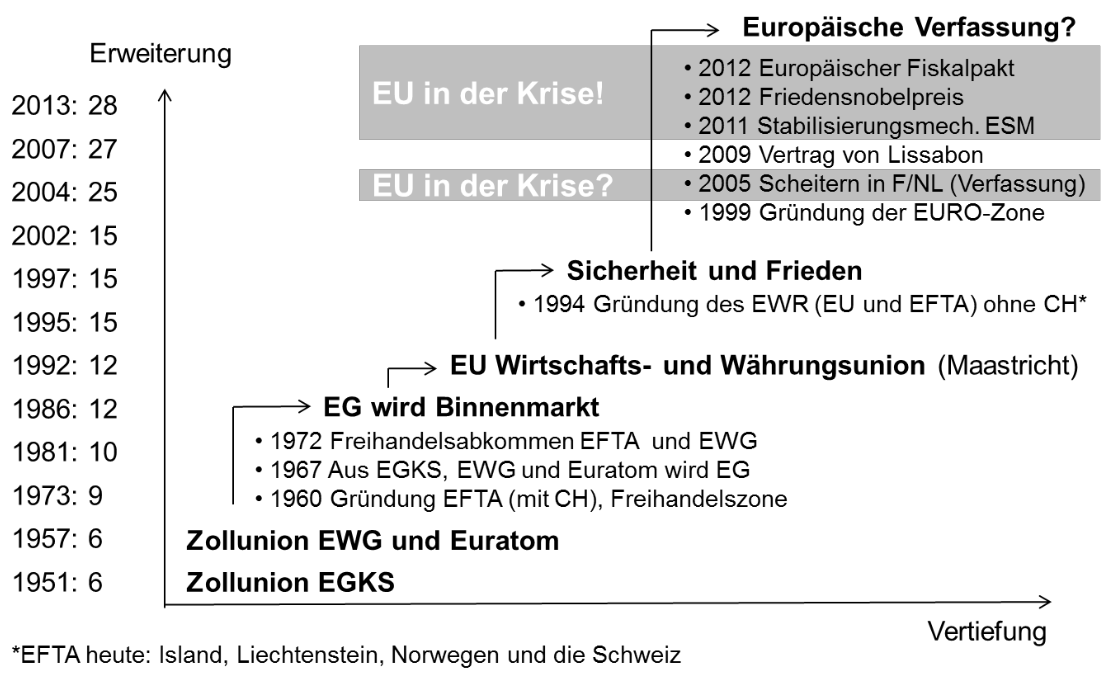
\includegraphics[width=.9\linewidth]{img/geschichte_eu.png}
\end{center}
\captionof{figure}{Geschichte der EU}\label{fig:geschichte-der-eu}
}

\subparagraph{Organe \& Struktur der EU} \
\label{sec:org1e431c9}
{
\begin{center}
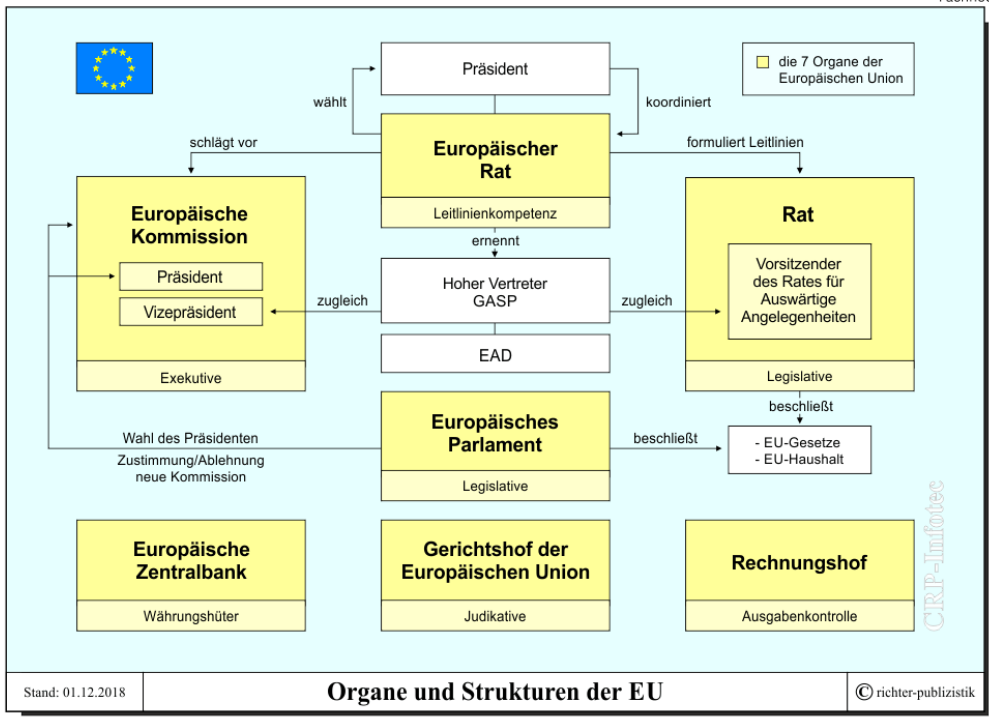
\includegraphics[width=.9\linewidth]{img/organe_und_strukturen_der_eu.png}
\end{center}
\captionof{figure}{Organe und Strukturen der EU}\label{fig:organe-und-strukturen-der-eu}
}

\section{{\bfseries\sffamily TODO} Aussenhandel Schweiz}
\label{sec:orge3c41ad}
\subparagraph{Aufbau Zahlungsbilanz} \
\label{sec:org55c715c}
{
\begin{center}
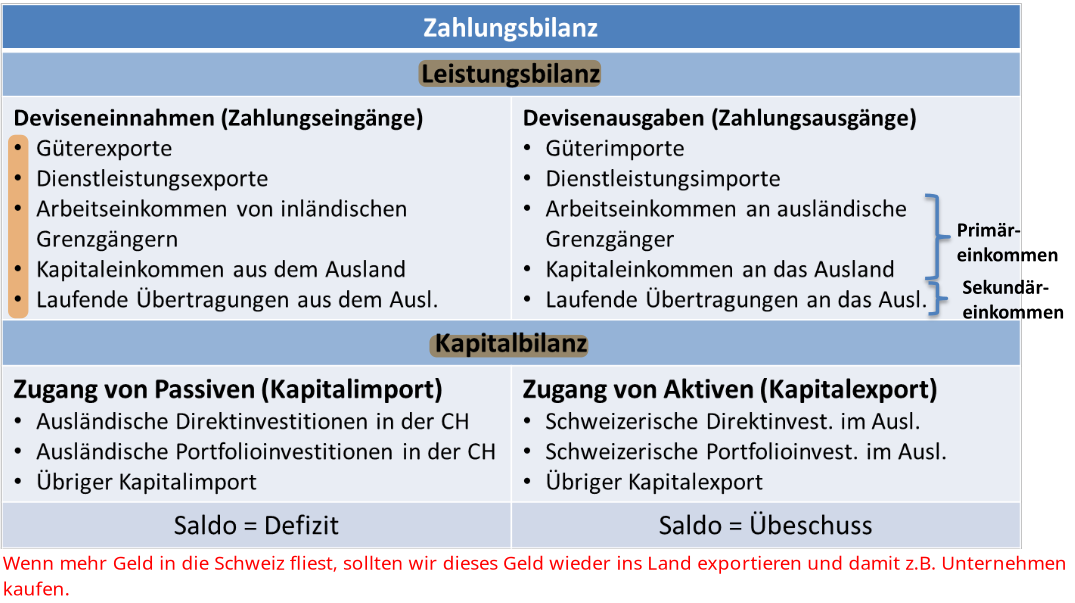
\includegraphics[width=.9\linewidth]{img/zahlungsbilanz.png}
\end{center}
\captionof{figure}{Aufbau einer Zahlungsbilanz}\label{fig:aufbau-einer-zahlungsbilanz}
}

\subparagraph{Intepretation Zahlungsbilanz} \
\label{sec:orgcf4ab91}
Bei einem Leistungsbilanzüberschuss:
\begin{itemize}
\item ist der Güterexport > Güterimport
\item Ausländische Touristen in der Schweiz > Schweizer Touristen im Ausland
\item Wir bieten mehr Leistung an, als wir selber vom Ausland nachfragen
\end{itemize}

Das bedeutet, dass das Land auf Konsum verzichtet (Gegenwartskonsum < Zukunftskonsum).

Bei einem Leistungsbilanzdefizit ist es genau umgekehrt, wir fragen nach mehr Güter als wir exportieren.

\section{General}
\label{sec:orgeed3f62}

{
\begin{center}
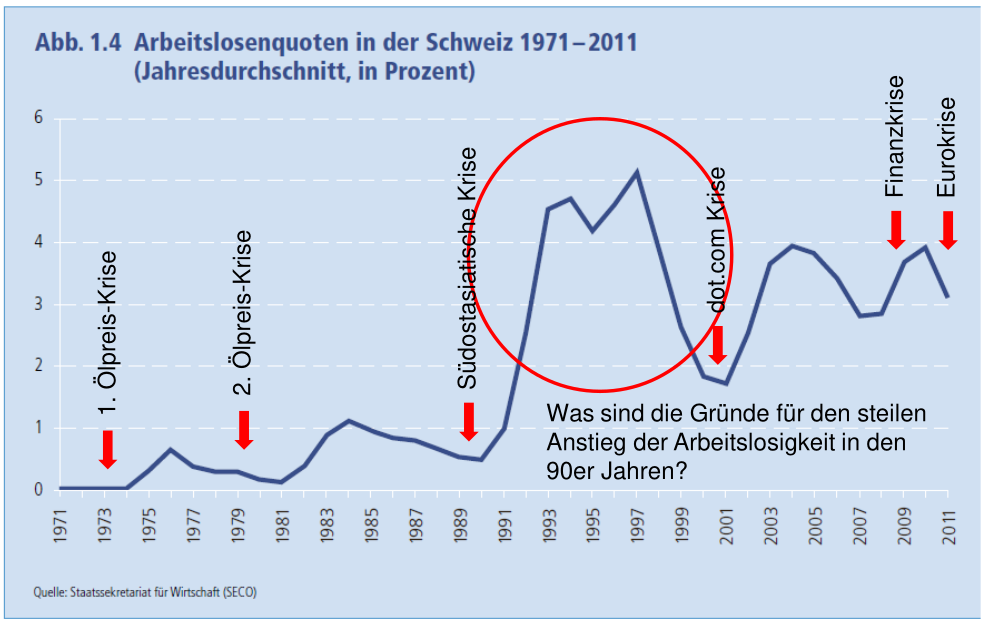
\includegraphics[width=.9\linewidth]{img/wirtschaftskrisen.png}
\end{center}
\captionof{figure}{Wirtschaftskrisen bis 2011}\label{fig:wirtschaftskrisen}
}

\end{multicols}
\end{document}